
% die Standard-Dokumentenklasse
\documentclass[11pt,a4paper]{article} %% 1.Ebene = chapter, headings

% input encoding, font encoding, outline font
\usepackage[utf8]{inputenc} 
\usepackage[T1]{fontenc} 
\usepackage{lmodern}
\usepackage{tcolorbox}
% Sprache
\usepackage[german]{babel}
\usepackage[section]{placeins}

% Absatzformatierung
\setlength{\parindent}{0pt}
\setlength{\parskip}{1ex plus 0.5ex minus 0.5ex}

% erweiterte mathematische Symbole
\usepackage{amsmath} 

% für Abbildungen
\usepackage{graphicx} 

% für Tabellen
\usepackage{booktabs}

% für Hyperlinks
\usepackage{hyperref}
\hypersetup{
	colorlinks,
	citecolor=red,
	filecolor=black,
	linkcolor=black,
	urlcolor=black}
\graphicspath{}

\graphicspath{}




\begin{document}

	

{
	\centering 
	\large 
	Physiklabor für Anfänger*innen \\
	Ferienpraktikum im Sommersemester 2018 \\[4mm]
	\textbf{\LARGE 
		Versuch 31: Mischungsmethode in der Kalorimetrie
	} \\[3mm]
	(durchgeführt am 12.09.2018 bei Nico Strauß) \\
	Ye Joon Kim, Marouan Zouari\\
	\today \\[10mm]
}

\tableofcontents
\section{Einleitung}
Die Wärmekapazität ist das Verhältnis der einem Körper zugeführte Wärme zu seinem Temperaturerhöhung. Bei Experimenten mit Kalorimeter ist es oft hilfreich die Wärmekapazität des Kalorimeters zu kennen, damit bessere Ergebnisse bekommen werden können. 

Aber, es gibt auch Ausnahme, wobei die Temperatur trotz Energiezufuhr sich nicht erhöht. Bei Phasenübergänge verursacht die Aufnahme oder Abgabe von Wärme keine Temperaturänderung. Die latente Wärme quantifiziert die Menge Wärme, die bei einem Phasenübergang aufgenommen oder abgegeben wird, ohne die Temperatur zu ändern. Insbesondere ist die latente Wärme beim Schmelzen auch als Schmelzwärme bezeichnet. 


\section{Ziel des Versuchs}
Das Ziel dieses Versuchs ist es, mit der Mischungsmethode verschiedene physikalische Werte zu bestimmen. 

In dem ersten Versuchsteil wird die Mischungsmethode verwendet um die Wärmekapazität eines Kalorimeters zu bestimmen.

 In dem zweiten Teil wird die Schmelzwärme von Eis bestimmt. 

\section{Aufbau}
Der Aufbau f\"ur diese Experiment besteht aus 3 wicnhtige komponenten :
\\\
\textbf{Das Kalorimeter}, wo das Mischen der Flüssigkeiten stattfinden.
\\\
\textbf{Ein elektrisches Thermometer}, das die Temperatur durch elektrischen Strom, der von dem Temperaturwechsel verursacht wird, bestimmt.
\\\
\textbf{Ein Computer mit dem Programm LabVIEW}, der die Konversion und das Aufnehmen der Daten erm\"oglicht .

 
\begin{figure}
	\centering
	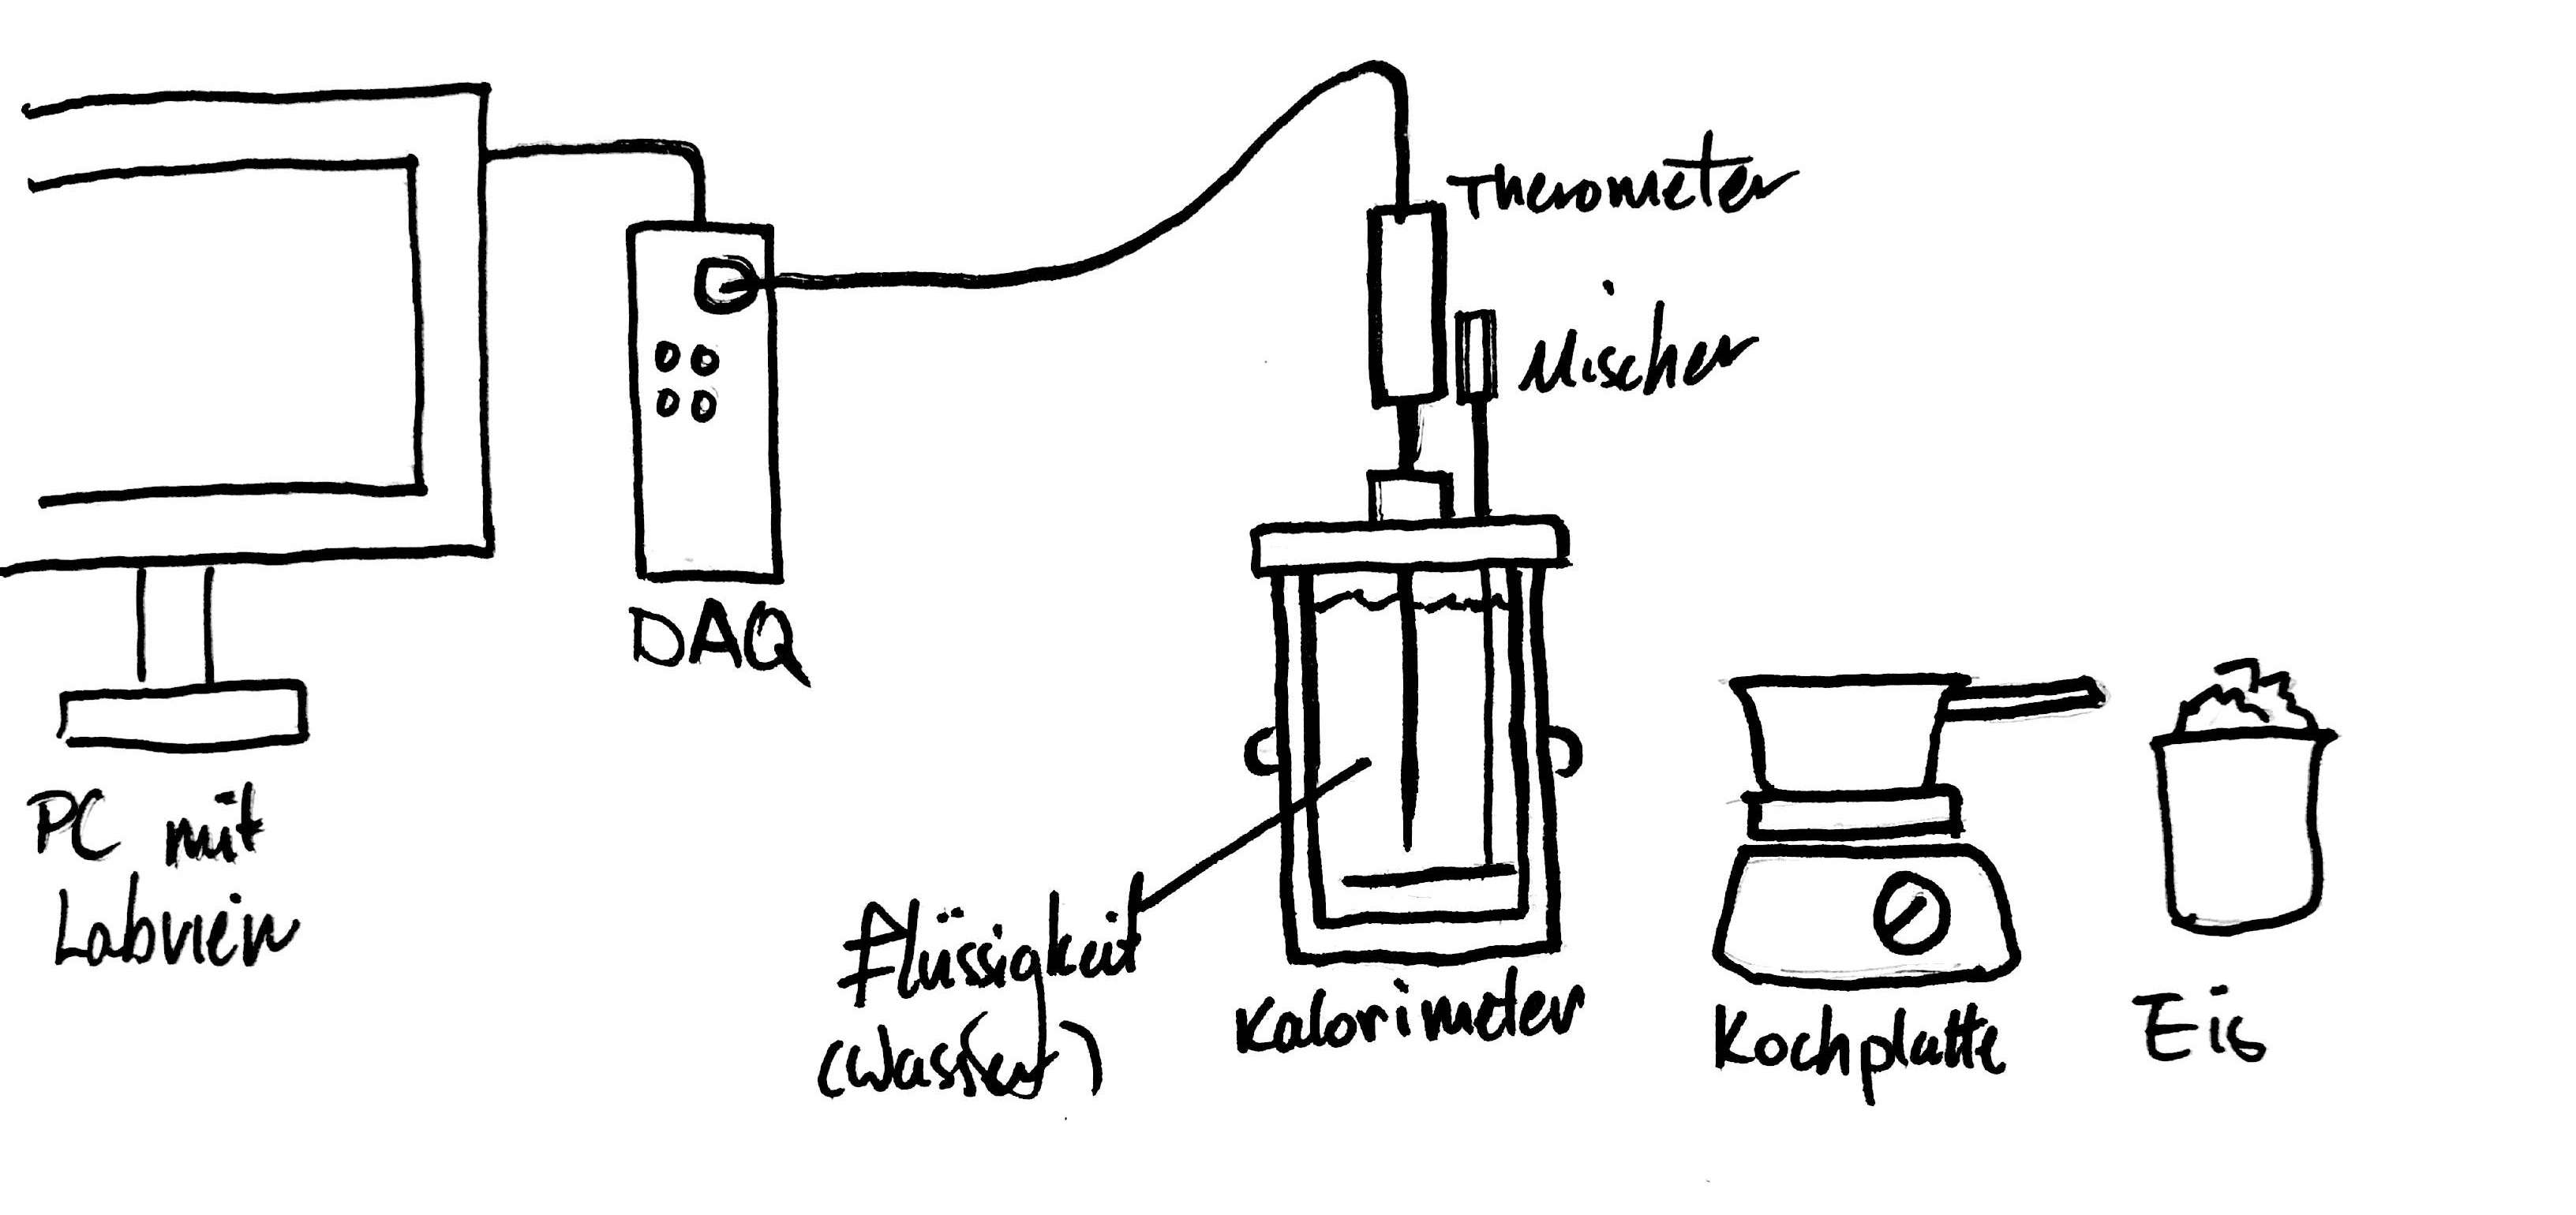
\includegraphics[width=\linewidth]{Abb3}
	\caption{Aufbau zu beiden Versuchsteilen}
\end{figure}

\section{Versuchsdurchf\"urhrung}

In für diesen Versuch muss das Programm zur Auswertung und Aufnahme zuerst kalibriert werden.
\\\
Zur Kalibrierung wurde Eis und kochendes Wasser verwendet. Zuerst wurde die Temperatur von Eis mit dem Thermometer gemessen. Für die akkurate Messung von 0 $^\circ$C wurde es gewartet, bis das Eis ein bisschen geschmolzen war, damit eine Eis-Wasser Mischung entstanden war. Die Abweichung von 0 $^\circ$C wurde dann von dem Messwert subtrahiert, damit der Apparat 0 $^\circ$C genau misst. 
Dann wurde die Temperatur des kochendes Wasser gemessen. Sei $T$ der gemessene Wert. Die Messwerte wurden dann mit $\frac{100}{T}$ multipliziert, um die Messungen zu 'Skalieren'. Dadurch sind die Messwerte für 0 $^\circ$C und 100 $^\circ$C akkurat, und deshalb der Thermometer kalibriert. 

\textbf{In dem 1. Teil } geht es um die Bestimmung der Wärmekapazität des Kalorimeters durch die Aufstellung einer Wärmeenergiebilanz .Daf\"ur wurde  eine Wassermenge, $m_h$ , 
mit der Temperatur $T_h$, in das Kalorimeter gegossen.
Es wurde gewartet, bis die in dem Programm gezeigte Temperatur zirka Konstant war. Danach wurde eine Wassermenge ,$m_k$ ($m_k < m_h$),  mit der Temperatur $T_k$ ,($T_k$<$T_h$), hinzugef\"ugt.
\\\
Ein st\"andiges Mischen mit dem Mischer war notwendig, um eine Mischung mit möglichst homogener Temperatur zu gewährleisten.
Nachdem die Temperatur wieder stabil war, wurde die erhaltenen Daten aufgenommen und mit dem Extrapolationsverfahren wurde $T_M$ berechnet. 
\\\
Der gesamte Prozesse wurde 3 mal wiederholt, um m\"ogliche statistische Fehler zu verringern. 

\textbf{Für die Bestimmung der Schmelzw\"arme von Eis} wurde eine Wassermenge ,$m_W$, mit der Temperatur $T_W$ in das Kalorimeter gegossen. Als die gemessene Temperatur innerhalb des Kalorimeters stabil war, wurde eine Eismenge ,$m_{eis}$, mit Temperatur $T_{eis}$ ($T_{eis}=0 ^oC$) hinzugef\"ugt.
\\\
Die Wassermenge soll ausreichend sein, um das Eis schmelzen zu können.
\\\
Hier ist ein st\"andiges Mischen f\"ur den gleichen Grund wie im 1. Teil notwendig.
Die Daten wurden nach der Stabilisierung der Temperatur innerhalb des Kalorimeters (deshalb als die Eisstücke vollständig geschmolzen waren) aufgenommen und die Werte für $T_M$ wurden mit dem Extrapolationsverfahren bestimmt.
Um statistische Fehler zu verringern wurden 3 Messereihe durchgef\"uhrt.



 \section{Auswertung und Fehleranalyse}

\subsection{1. Versuchsteil: Bestimmung der Wärmekapazität des Kalorimeters}

Zur Bestimmung der Wärmekapazität des Kalorimeters wird die folgende Wärmeenergiebilanz benutzt:

\begin{equation}
 \Gamma_\textrm{Kal} = c_\textrm{W}(m_\textrm{k}\beta-m_\textrm{h})  \quad \textrm{mit} \quad \beta = \frac{T_M-T_k}{T_h-T_M}
\end{equation}

\textbf{Die  Werte von $T_M$} wurden durch das Extrapolationsverfahren erhalten.Und Für das Extrapolationsverfahren wurde das Photoshop\textregistered \ Programm von Adobe benutzt: 

Eine Kurve wurde mit dem Pen-tool gezeichnet, die den Temperaturverlauf modelliert. Dann wurde eine Senkrechte Linie eingezeichnet nach dem Zeitpunkt, wo das kalte Wasser in das Kalorimeter gegossen wurde. 
Mit dem Lasso-Tool kann die Gebiete zwischen die Kurve und die Linie ausgewählt und deren Flächen berechnet werden. Die Linie wurde bewegt, bis beide Gebiete schätzungsweise gleich waren.

\textbf{Die Unsicherheiten bei der Temperatur} wurden von dem Diagramm abgeschätzt. 

Siehe Abbildungen 2,3 auf n\"achster Seite.

Die Werte für die drei Messereihe sind :

\begin{table}[h]
	\centering
	\begin{tabular*}{0.99\textwidth}{@{\extracolsep{\fill}}cccccc}
		\toprule
		Messreihe & $T_M$ & $\Delta T_M$  \\
		& $^\circ$ C & $^\circ$ C \\
	    \bottomrule
		1 & 43 & 2  \\
		2 & 23 & 2 \\
		3 & 61 & 2 \\
		\bottomrule
	\end{tabular*}
	\caption{Die berechneten Mischungstemperaturen und deren   Unsicherheiten.}
	\label{tabelle}
\end{table}
\newpage
\begin{figure}[h]
\centering
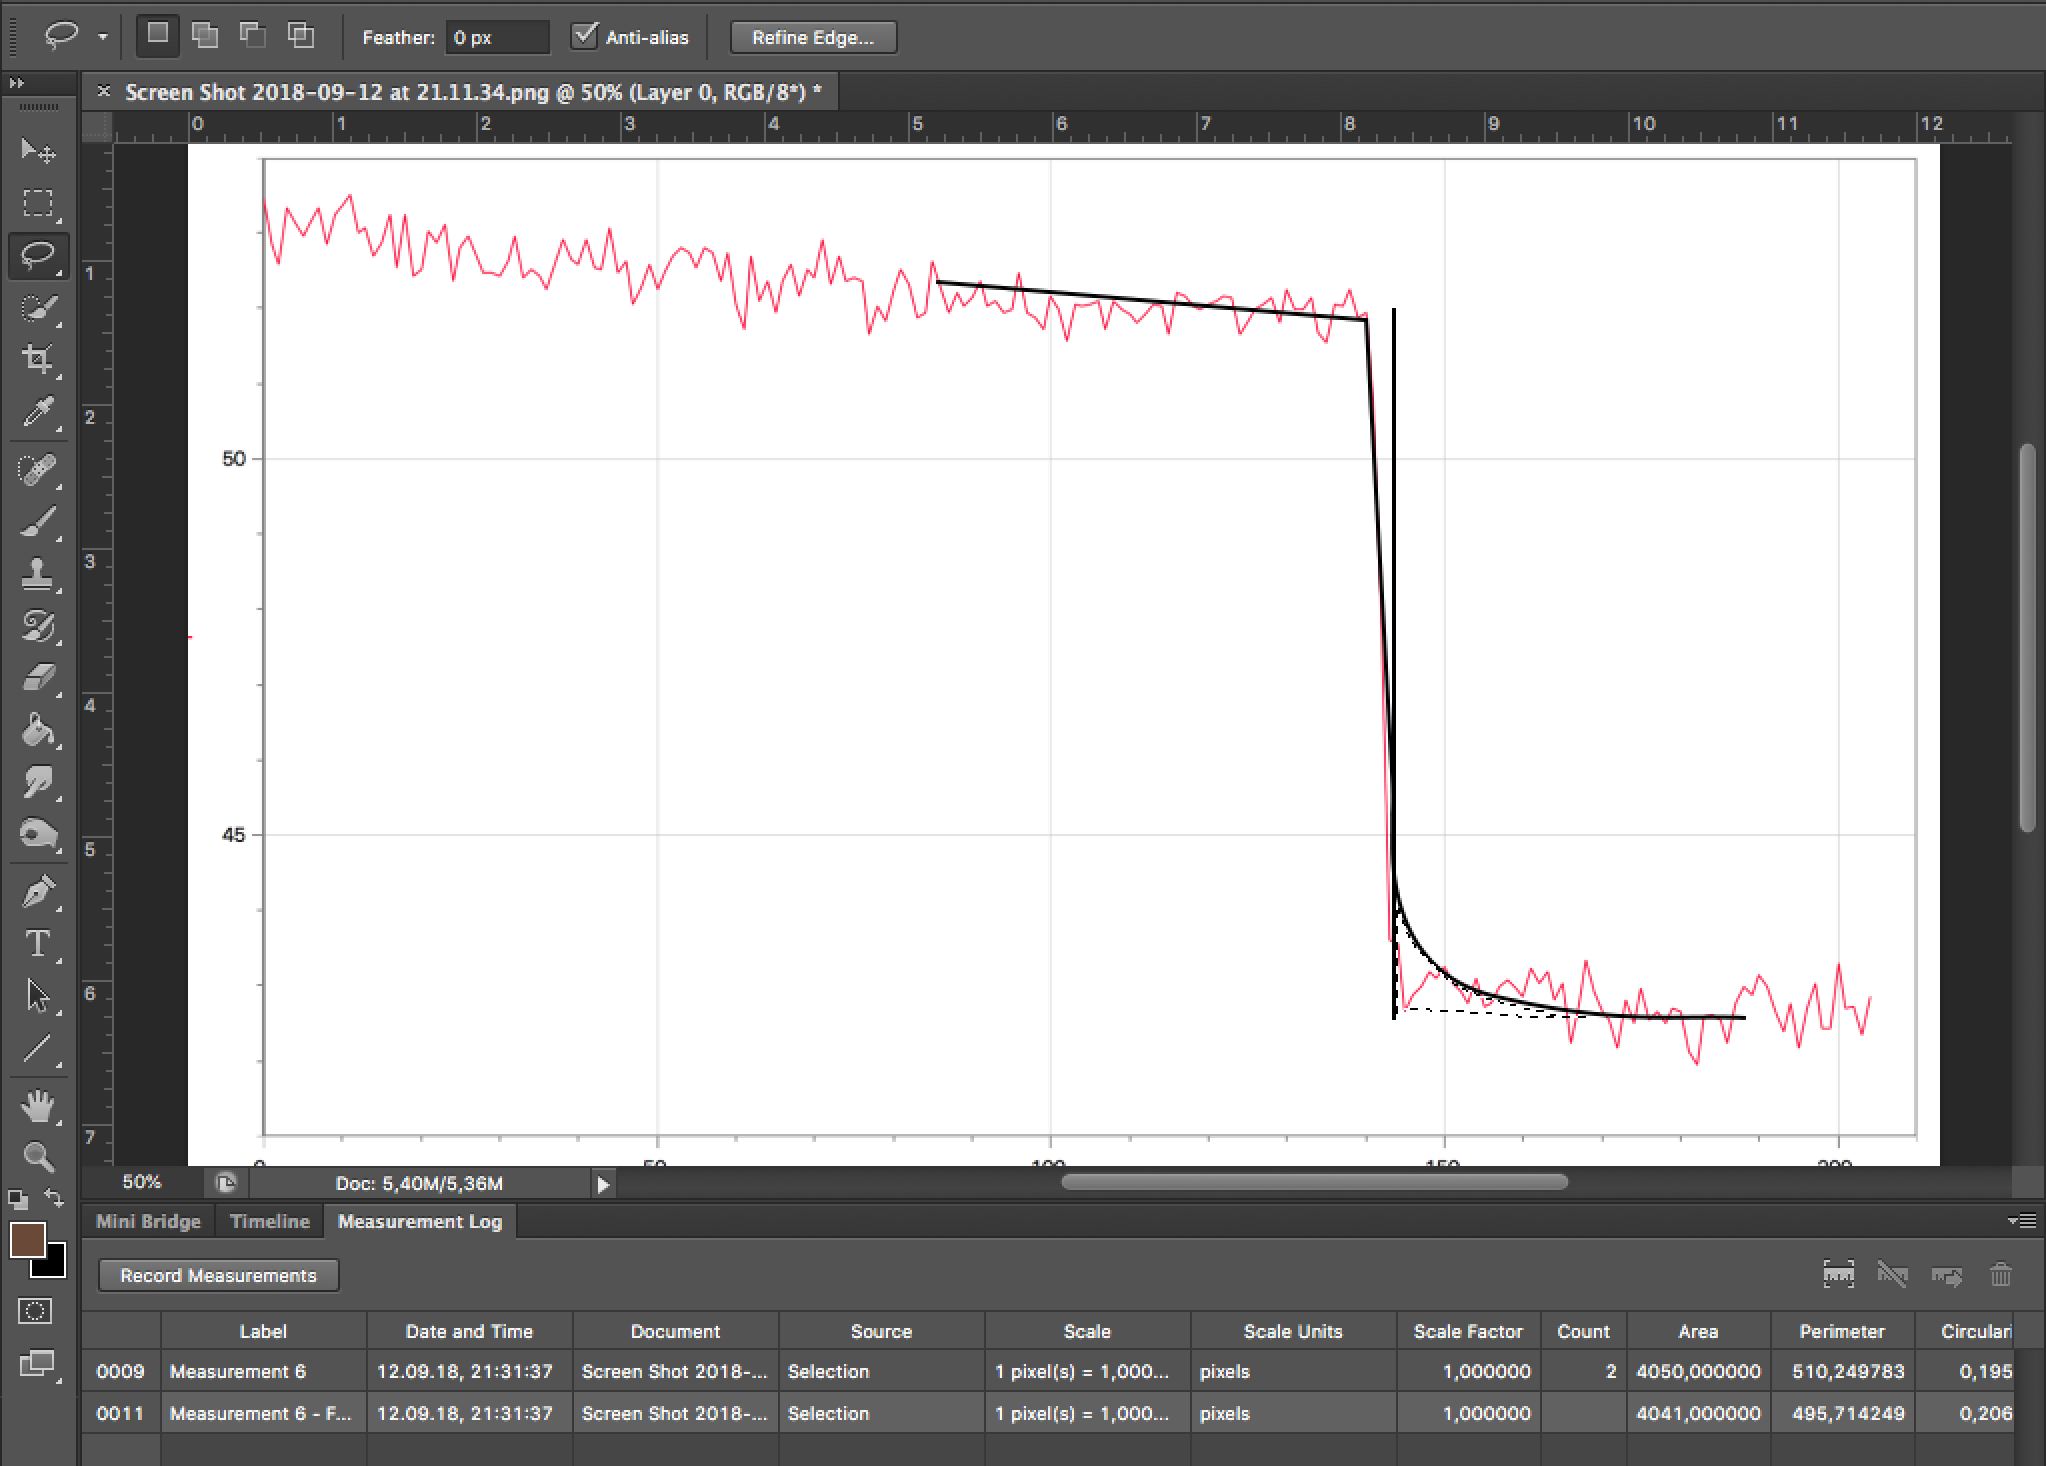
\includegraphics[width=\linewidth]{Abb1}
\caption{Benutzung von Photoshop um die Fläche von beide Gebiete vor und nach der Senkrechte Strecke zu bestimmen}
\end{figure}

\begin{figure}[h]
\centering
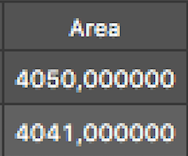
\includegraphics{Abb2}
\caption{Vergleich der Flächen beider Gebiete. (Einheiten in Pixels)}
\end{figure}

\newpage	

Jetzt lassen sich die Werte für $\Gamma_\textrm{Kal}$ mit den Werten für $T_h$, $T_k$, $m_k$, und $m_h$ bestimmen. Die Werte von $\Gamma_\textrm{Kal}$ für die drei Messreihen sind:

\begin{table}[h]
	\centering
	\begin{tabular*}{0.99\textwidth}{@{\extracolsep{\fill}}cccccc}
		\toprule
		Messreihe & $\Gamma_\textrm{Kal}$ & $\Delta \Gamma_\textrm{Kal}$  \\
		& J / K & J/ K\\
		\bottomrule
		1 & 107 & 95  \\
		2 & 126 & 176 \\
		3 & 15 & 73 \\
		\bottomrule
	\end{tabular*}
	\caption{Die Wärmekapazität des Kalorimeters und deren Unsicherheiten.}
	\label{tabelle3}
\end{table}

\textbf{Für die Berechnung der Unsicherheit $\Delta \Gamma_\textrm{Kal}$} wurden die Gauß'sche Fehlerfortpflanzung benutzt.  mit:
$$f(m_k, m_h, T_M, T_k, T_h) = c_\textrm{W}(m_\textrm{k} \frac{T_M-T_k}{T_h-T_M} -m_\textrm{h}) $$
$$ \frac{\partial f}{\partial m_k} = c_W\frac{T_M-T_k}{T_h-T_M}$$
$$ \frac{\partial f}{\partial m_h} = c_W$$
$$ \frac{\partial f}{\partial T_h} = -c_W m_k \frac{T_M - T_k}{(T_h-T_M)^2} $$
$$ \frac{\partial f}{\partial T_k} = \frac{-c_W m_k}{T_h-T_M} $$
$$ \frac{\partial f}{\partial T_M} = c_W m_k \frac{T_h-T_k}{(T_M-T_h)^2} $$

Aber da $\frac{\partial f}{\partial T_M} \Delta T_M$, $\frac{\partial f}{\partial T_h} 
\Delta T_h$ und $\frac{\partial f}{\partial T_k} \Delta T_k$ überwiegend größer als die anderen Terme 
(mindestens dreimal größer) sind, wurden die Unsicherheit berechnet als:
$$\Delta \Gamma_\textrm{Kal} = \sqrt{(\frac{\partial f}{\partial T_M} \Delta T_M)^2+(\frac{\partial f}{\partial T_h} \Delta T_h)^2+(\frac{\partial f}{\partial T_k} \Delta T_k)^2 }$$


\textbf{Der Mittelwert} und seine Unsicherheit (Standardabweichung) lauten:
$$(83 \pm 60 ) \textrm{J / K}$$

\subsection{2. Versuchsteil: Bestimmung der Schmelzwärme von Eis}

Die Schmelzwärme von Eis (mit $q_\textrm{Eis}$ bezeichnet) lässt sich mit der folgenden Formel bestimmen:


\begin{equation}
q_\textrm{Eis} = \frac{(m_W c_W + \Gamma_\textrm{Kal})(T_W - T_M) - m_\textrm{Eis} c_W(T_M - T_\textrm{Eis})}{m_\textrm{Eis}}
\end{equation}

Die Werte für $T_M$ lassen sich wiederum mit dem obigen Extrapolationsverfahren (in Teil 4.1) bestimmen:

\begin{table}[h]
	\centering
	\begin{tabular*}{0.99\textwidth}{@{\extracolsep{\fill}}cccccc}
		\toprule
		Messreihe & $T_M$ & $\Delta T_M$  \\
		& $^\circ$ C & $^\circ$ C \\
		\bottomrule
		1 & 25 & 2  \\
		2 & 32 & 2 \\
		3 & 38 & 2 \\
		\bottomrule
	\end{tabular*}
	\caption{Die Mischungstemperaturen und deren Unsicherheiten}
	\label{tabelle2}
\end{table}

Die Werte für $T_M$ eingesetzt in Formel (2) liefert:

\begin{table}[h]
	\centering
	\begin{tabular*}{0.99\textwidth}{@{\extracolsep{\fill}}cccccc}
		\toprule
		Messreihe & $q_\textrm{Eis}$ & $\Delta q_\textrm{Eis}$  \\
		& J / kg & J / kg \\
		\bottomrule
		1 & $668,4\cdot10^{3}$ & $10^{3}$  \\
		2 & $110\cdot10^{3}$ & $96\cdot10^{3}$ \\
		3 & $21\cdot10^{3}$ & $22\cdot10^{3}$ \\
		\bottomrule
	\end{tabular*}
	\caption{Die berechneten Werte für die Schmelzwärme von Eis}
	\label{tabelle4}
\end{table}

\textbf{Für die Unsicherheiten $\Delta q_\textrm{Eis}$ }wurde die Gauß'sche Fehlerfortpflanzung benutzt. Mit:
$$f(m_W,\Gamma_\textrm{Kal},T_W, T_M, m_\textrm{Eis}) $$ 
$$ = \frac{(m_W c_W + \Gamma_\textrm{Kal})(T_W - T_M) - m_\textrm{Eis} c_W(T_M - T_\textrm{Eis})}{m_\textrm{Eis}} $$
sind:
$$ \frac{\partial f}{\partial m_W} = \frac{c_W(T_W-T_M)}{m_\textrm{Eis}}$$
$$ \frac{\partial f}{\partial \Gamma_\textrm{Kal}} = \frac{T_W-T_M}{m_\textrm{Eis}}$$
$$ \frac{\partial f}{\partial T_W} = \frac{m_W c_W + \Gamma_\textrm{Kal}}{m_\textrm{Eis} }$$
$$ \frac{\partial f}{\partial T_M} = \frac{m_W c_W + \Gamma_\textrm{Kal} - m_\textrm{Eis} c_W}{m_\textrm{Eis}} $$
$$\frac{\partial f}{\partial m_\textrm{Eis}} = \frac{m_W c_W + \Gamma_\textrm{Kal}}{m_\textrm{Eis}^2}$$
Aber da der Betrag von $\frac{\partial f}{\partial \Gamma_\textrm{Kal}} \Delta \Gamma_\textrm{Kal}$ mindestens dreimal größer war als alle andere Beträge, wurden die anderen Beträge vernachlässigt. 
Die Unsicherheiten der Werte für $q_\textrm{Eis}$ sind dann durch
$$\Delta q_\textrm{Eis} = \frac{\partial f}{\partial \Gamma_\textrm{Kal}} \Delta \Gamma_\textrm{Kal}$$
zu bestimmen.

\textbf{Der Mittelwert} der Werte und seine Unsicherheit (Standardunsicherheit) ist dann:
$$(330\cdot10^{3} \pm 290\cdot10^{3}) \textrm{J/K}$$

\section{Diskussion der Ergebnisse}
\subsection{Systematische und statistische Fehler :}

Bei beiden Teile k\"onnten verschiedene statistische und
systematische Fehler auftauchen.
\\\
\textbf{In dem 1. Teil} wurde kochendes und heißes Wasser benutzt.
Die gemessene Wassermenge kann nicht konstant sein, da ein Teil davon als Dampf verloren geht. Dadurch entsteht ein statistischer Fehler bei den Werten für $m_h$.
Ein anderer statistischer Fehler stammt von der Unterbrechung der Isolierung des Kalorimeters bei dem Einfüllen der zweiten Wassermenge.
\\\
Außerdem ist es angenommen, dass das Kalorimeter verlustfrei ist. Das stimmt in der Wirklichkeit nicht, wodurch ein systematischer Fehler entsteht, da die gemessene Temperatur immer größer als die reelle Temperatur ist. 

\textbf{In dem 2. Teil} wurde angenommen, dass das Eis eine anfängliche Temperatur von $0^oC$ hat, aber in der Realit\"at könnte es der Fall sein, dass das Wasser nicht 100\% reines Wasser ist. Deswegen sind die Werte von $q_\textrm{Eis}$, die durch die Formel
$q_\textrm{Eis} = \frac{(m_W c_W + \Gamma_\textrm{Kal})(T_W - T_M) - m_\textrm{Eis} c_W(T_M - T_\textrm{Eis})}{m_\textrm{Eis}}$ berechnet wurden, eine Angleichung. Dies f\"uhrt zu einem systematischen Fehler.
\\\
Darüber hinaus sind eventuelle Kontakte zwischen dem Mischer und dem elektrischen Thermometer beim Mischen, als auch die Unterbrechung der Isolierung des Kalorimeters beim Einf\"ullen vom Eis Ursprünge von statistischen Fehler.

\subsection{Diskussion \"uber die gefundene Werten :}

\textbf{Bei dem ersten Teil dieses Versuchs} ist  die berechnete W"armekapazit"at des Kalorimeters gleich $$(83 \pm 60 ) \mathrm{\frac{J}{K}}.$$
Weil die Unsicherheit bei 75\% liegt ist der Wert nicht
von großer Bedeutung.
\\\
Gründe daf\"ur k\"onnten die vorher erwähnten statistischen und systematischen Fehler sein.

\textbf{Die berechnete Schmelzw\"arme von Eis} lautet:
$$(330\cdot10^{3} \pm 290\cdot10^{3}) \mathrm{\frac{J}{K}}$$
$$=(330 \pm 290) \mathrm{\frac{kJ}{K}}$$
Der Wert liegt sehr nah am  Literaturwert, der $(333,5\cdot10^{3}\mathrm{\frac{J}{K}}$ ist (,,Enthalpy of Fusion'').
Jedoch ist die Unsicherheit des Wertes selbst $88\%$, also ist das Ergebnis nicht von gro{\ss}er Signifikanz. Deswegen kann das Ergebnis dieses Teils des Versuchs nicht als Nachweis für den Literaturwert genommen werden.

\subsection{M"ogliche Methoden zur Verbesserung der Experiment: }

Um die Isolierung des Kalorimeters besser zu bewahren, könnte das Eis in kleineren Stücken mit bekannten Massen vorbereitet sein, sodass es durch eine kleinere Öffnung in einer kürzeren Zeit in das Kalorimeter eingef\"ullt werden könnte.
\\\
Das selbe gilt auch f\"ur den ersten Teil.

Außerdem sollte berücksichtigt werden, dass das Wasser nicht 100\% destilliertes Wasser ist, und deshalb die anf\"angliche Temperatur des Eises nicht genau gleich $0^{\mathrm{o}}$C ist. Deshalb sollte eine verallgemeinerte Formel f\"ur die Bestimmung von $q_{eis}$ benutzt werden.




\section{Literatur}

\section{Anhang: Rohe Daten}

\end{document}